\documentclass[12pt]{article}
\usepackage[a4paper, total={5.5in, 9in}]{geometry}
\usepackage{amsmath}
\usepackage{changepage}
\usepackage[most]{tcolorbox}
\usepackage{textcomp}
\usepackage{tikz}
\usepackage{pgfplots}
\pgfplotsset{compat=1.18}
\usepackage{amsfonts}
\usepackage{graphicx}

\newcommand{\ihat}{\boldsymbol{\hat{\textbf{\i}}}}
\newcommand{\jhat}{\boldsymbol{\hat{\textbf{\j}}}}


\title{Precalculus Worksheet 10.1}
\author{PCL Learning Center}
\date{}

\begin{document}
\maketitle

\begin{center}
    \textit{note: No graphing calculators or electronic devices may be used on this worksheet.}    
\end{center}

\section*{Problem Set 1\\Difficulty level: Normal}
\subsection*{Problem 1}
What are the coordinates of the co-vertices in the figure below?
\begin{figure}[!ht]
    \centering
    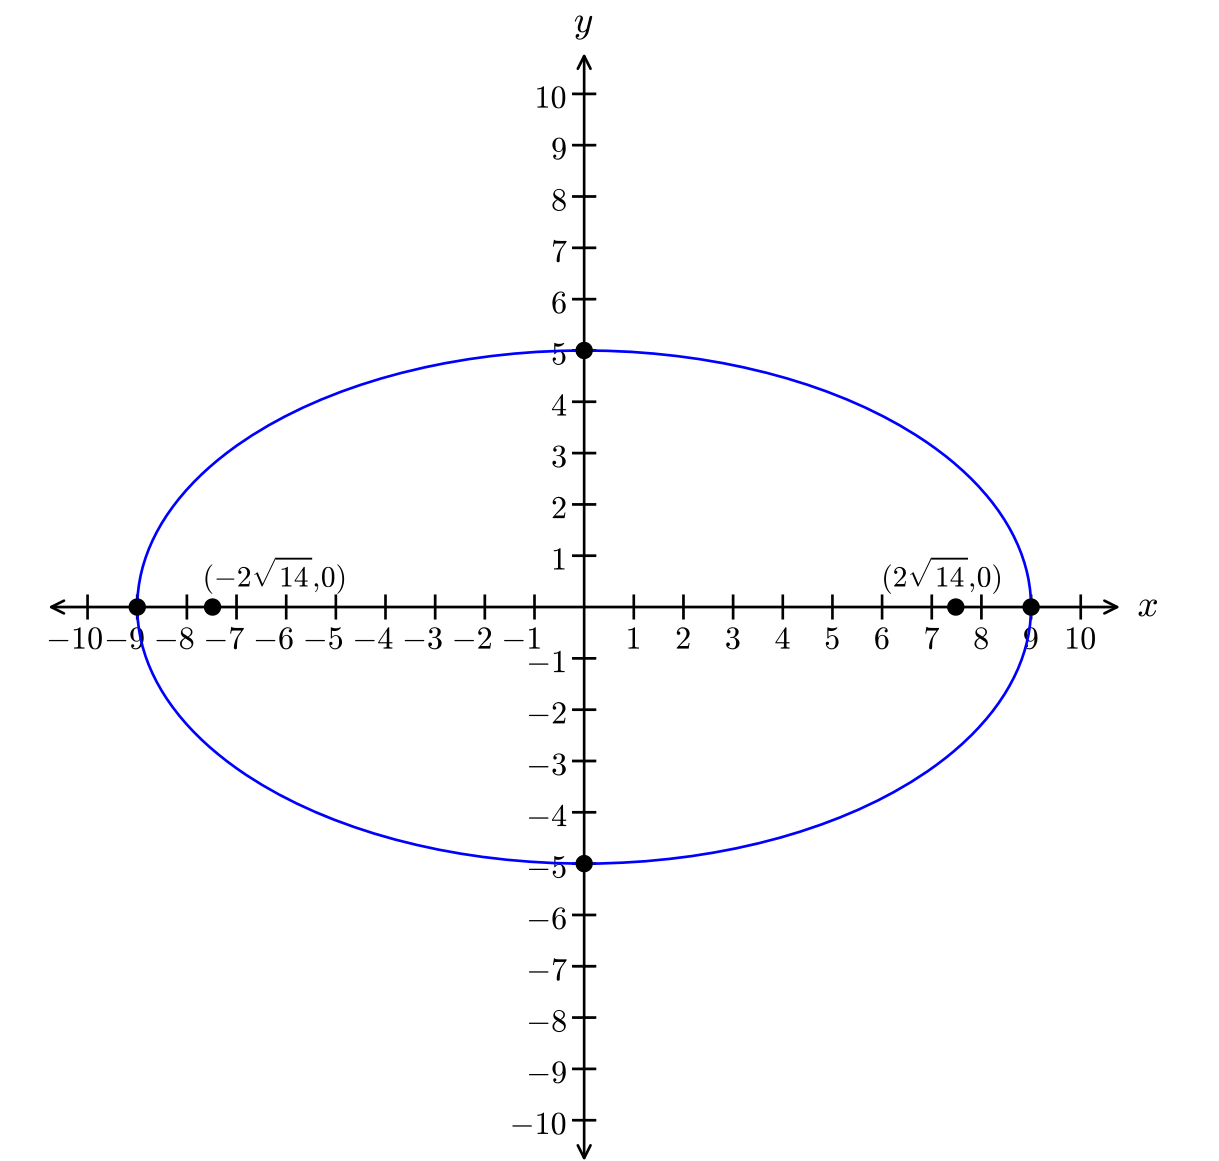
\includegraphics[width=0.9\linewidth]{1.png}
\end{figure}

\newpage
\subsection*{Problem 2}
Identify the coordinates of the co-vertices of the ellipse shown below.

\begin{figure}[!ht]
    \centering
    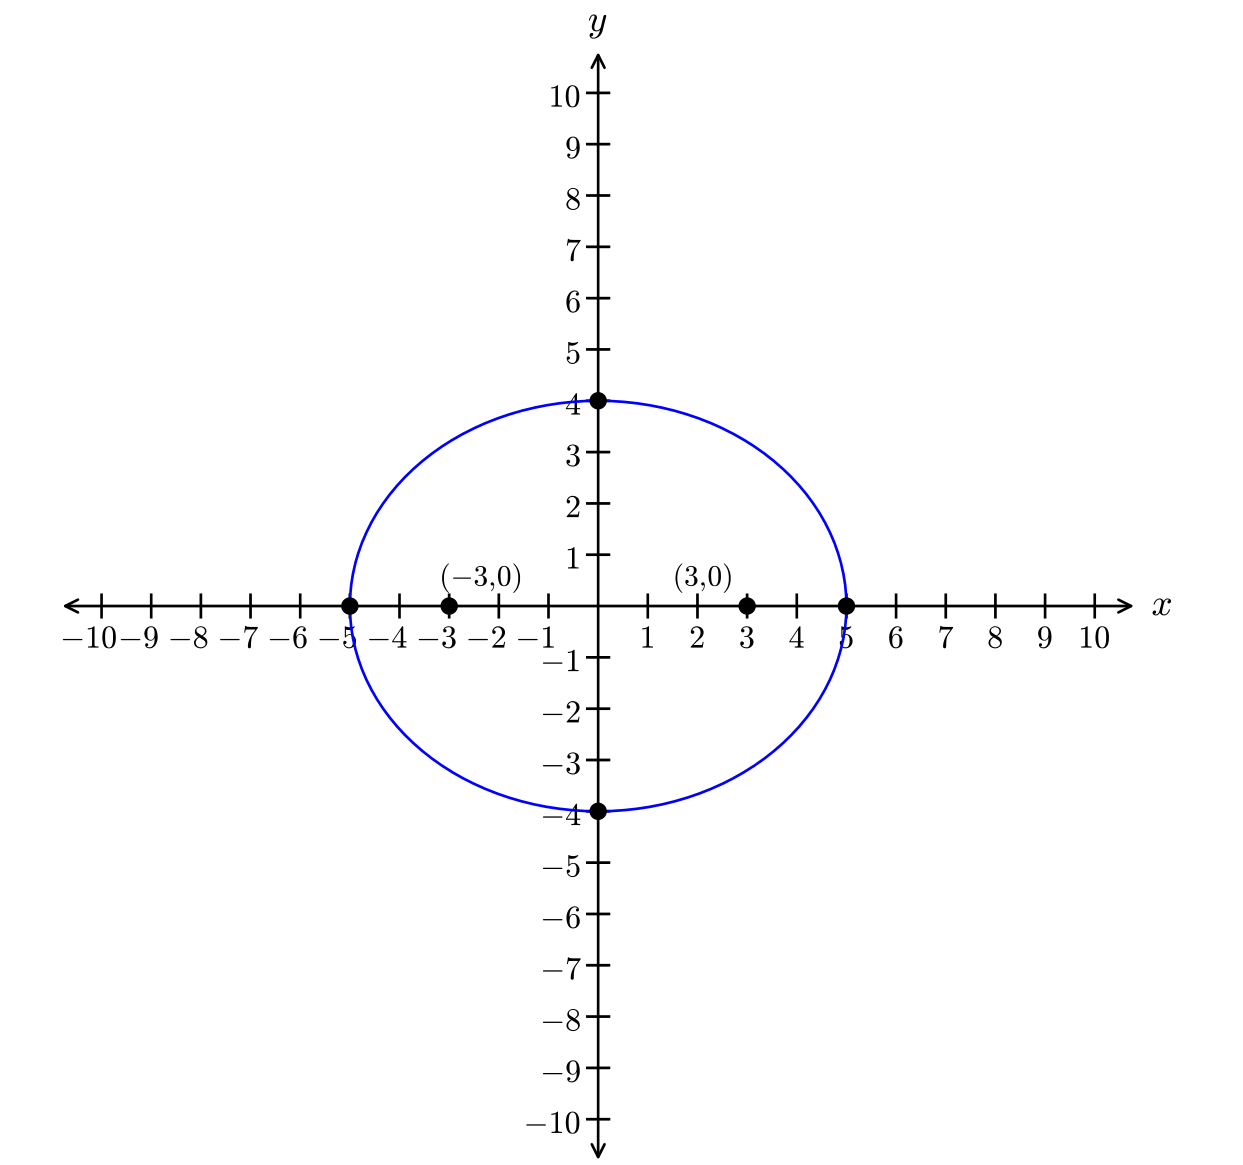
\includegraphics[width=1\linewidth]{2.png}
\end{figure}

\subsection*{Problem 3}
Determine the coordinates of the two foci given the ellipse,
\[\dfrac{x^2}{14}+\dfrac{y^2}{50}=1\]

\subsection*{Problem 4}
What is the direction of the minor axis and what is its length of the ellipse,
\[\dfrac{x^2}{49}+\dfrac{y^2}{25}=1\]

\subsection*{Problem 5}
What is the standard form equation of the ellipse that has vertices \((0, \pm 9)\) and co-vertices \((\pm 1,0)\)?

\subsection*{Problem 6}
Determine if the following are ellipses. If yes, write in standard form.
\begin{enumerate}
    \item[(a)] \[4x^2+9y^2=1\]
    \item[(b)] \[\dfrac{(x-2)^2}{49}+\dfrac{(y-4)^2}{25}=1\]
\end{enumerate}


\section*{Problem Set 2\\Difficulty level: Hard}
\subsection*{Problem 1}
Determine if the following equations represent ellipses. If yes, write in standard form.
\begin{enumerate}
    \item[(a)] \[4x^2-8x+9y^2-72y+112=0\]
    \item[(b)] \[x^2+2x+100y^2-1000y+2401=0\]
\end{enumerate}

\newpage
\section*{Solutions for the Set 1}
\subsection*{Problem 1}
\((0,-5),(0,5)\)
\subsection*{Problem 2}
\((0,-4),(0,4)\)
\subsection*{Problem 3}
\((0,-6),(0,6)\)
\subsection*{Problem 4}
The minor axis is along the \(y-\)axis and has length 10.
\subsection*{Problem 5}
\(x^2+\dfrac{y^2}{81}=1\)
\subsection*{Problem 6}
\begin{enumerate}
    \item[(a)] \[\dfrac{x^2}{\Big(\dfrac{1}{4}\Big)}+\dfrac{y^2}{\Big(\dfrac{1}{9}\Big)}=1\]
    \item[(b)] It is already given in standard form.
\end{enumerate}

\section*{Solutions for the Set 2}
\subsection*{Problem 1}
\begin{enumerate}
    \item[(a)] 
    \begin{align*}
    4x^2 - 8x + 9y^2 - 72y + 112 &= 0 \\
    4(x^2 - 2x) + 9(y^2 - 8y) &= -112 \\
    4[(x - 1)^2 - 1] + 9[(y - 4)^2 - 16] &= -112 \\
    4(x - 1)^2 + 9(y - 4)^2 &= 36 \\
    \dfrac{(x - 1)^2}{9} + \dfrac{(y - 4)^2}{4} &= 1
    \end{align*}

    \item[(b)] 
    \begin{align*}
    x^2 + 2x + 100y^2 - 1000y + 2401 &= 0 \\
    (x^2 + 2x) + 100(y^2 - 10y) &= -2401 \\
    (x + 1)^2 - 1 + 100[(y - 5)^2 - 25] &= -2401 \\
    (x + 1)^2 + 100(y - 5)^2 &= 100 \\
    \dfrac{(x + 1)^2}{100} + \dfrac{(y - 5)^2}{1} &= 1
    \end{align*}
\end{enumerate}


\end{document}
